\chapter{Proposta para análise de arquiteturas \ac{mmorpg}}
\label{cap3}



As arquiteturas de serviços \ac{mmorpg} são desenvolvidas visando suprir as necessidades do projeto do jogo desenvolvido, de forma a viabilizar a utilização deste serviço.
%
Nesse sentido, jogos com mecânicas de projeto similares possuem implementações parecidas para os clientes.
%
Entretanto, a arquitetura escolhida impacta no custo de operação e qualidade do serviço aos jogadores.
%
Por este motivo, diferentes arquiteturas com o mesmo \textit{design} não são comparáveis entre sí, visto que dependem das regras de negócio do jogo.



Ao desenvolver um serviço \ac{mmorpg} é necessário decidir uma arquitetura que possibilite reduzir custos, consumo de recursos e minimize ocorrências para os jogadores a fim de viabilizar a sua implantação como produto.
%
Porém, a impossibilidade de comparação direta entre as arquiteturas de serviço \ac{mmorpg} instiga a análise das características básicas destas arquiteturas que possam influenciar o \textit{game design}, tais como consumo de recursos, tempo de resposta, latência e número máximo de clientes simultâneos conectados nos microsserviços.
%
Sendo assim, uma análise do consumo de recursos computacionais das arquiteturas levantadas previamente na literatura tem valor científico no auxílio na escolha de implementações arquiteturas de microsserviços, em específico para serviços \ac{mmorpg}.



Nesta seção é descrito a proposta para análise de consumo de recursos computacionais em arquiteturas \ac{mmorpg}.
%
Inicialmente, é descrita a proposta em alto nível (Subseção~\ref{sec:proposta}), trazendo os objetivos desta análise, quais recursos e métricas serão analisadas (TCC-II).
%
Os Critérios de Análise (Subseção~\ref{sec:criterios}) exibem como os dados obtidos devem ser interpretados, baseando-se nos objetivos da análise das arquiteturas.
%
O Plano de Testes (Subseção~\ref{sec:plano}) exibe como será realizada a coleta dos dados, descrevendo ambiente, cenário, critérios e testes na qual serão realizados para obter os objetivos deste trabalho.
%

\section{Proposta}
\label{sec:proposta}

Tendo analisado os trabalhos relacionados (Seção~\ref{sec:similares}) e as arquiteturas específicas para jogos \ac{mmorpg}, o presente trabalho tem como objetivo analisar as arquiteturas \ac{mmorpg} visando complementar a análise de arquitetura e consumo de recursos computacionais não analisados nos trabalhos relacionados.
%
Em específico, serão obtidos os valores referentes aos recursos computacionais das arquiteturas Rudy (Subseção~\ref{rudy}), Salz (Subseção~\ref{salz}) e Willson (Subseção~\ref{willson}), conforme a Tabela~\ref{tab:recursos_categoria}:

\begin{enumerate}
  \item \textbf{\ac{cpu}}: o uso de CPU, com sua representação sendo em relação a porcentagem de processamento nos núcleos utilizados;
  \item \textbf{Memória}: Quantidade de memória utilizada pelos processos do serviço/arquitetura. A sua representação será como dado absoluto;
  \item \textbf{Rede}: Banda de rede utilizada nas operações de entrada e saída para cada microsserviço, utilizando valores absolutos. Também será obtido o valor de latência do cliente ao microsserviço, verificando se o congestionamento da rede afeta a latência do microsserviço.
\end{enumerate}

Além dos recursos computacionais, esta análise levará em conta valores referentes a outras métricas.
%
As métricas, cujos os valores serão obtidos são:

\begin{enumerate}
  \item \textbf{Número máximo de jogadores simultâneos}: Descobrir o limite de conexões para as arquiteturas propostas a análise. Será representado como valor absoluto.
  \item \textbf{Tempo de resposta das requisições}: Descobrir o tempo de resposta por categoria de requisição, conforme o número de jogadores no serviço. Será representado como tempo decorrido, em milissegundos.
\end{enumerate}

Todos estes valores serão obtidos a partir de simulações, e por este motivo faz-se necessário descrever o comportamento dos jogadores simulados.
%
Espera-se em situações adversas, caracterizar os comportamentos das arquiteturas, gargalos e os custos de recursos computacionais para manutenção das arquiteturas de microsserviços.
%
Para este fim, faz-se necessário a descrição dos critérios que serão utilizados durante a análise dos valores obtidos nos experimentos.

%ccm
% objetivos
% Definição das métricas para os itens levantados nas Tabelas 2.4 e 2.5

\section{Critérios de análise}
\label{sec:criterios}

A fim de padronizar a análise dos dados obtidos, a seção Critérios de Análise irá descrever como será guiada a análise conforme o comportamento dos valores obtidos.
%
Neste sentido, a análise dos dados obtidos serão guiadas pelo esperado dos valores obtidos em um serviço perfeito: %ccm o quê é um serviço perfeito? footnote

\begin{enumerate}
  \item \textbf{Consumo CPU}: Espera-se estressar com um elevado número de requisições.
  \item \textbf{Consumo Memória}: Espera-se estressar com requisições na qual exija armazenamento em memória.
  \item \textbf{Vazão Rede - Entrada}: Espera-se estressar com requisições na qual tenham uma carga de dados elevada.
  \item \textbf{Vazão Rede - Saída}: Espera-se estressar com respostas na qual tenham uma carga de dados elevada.
  \item \textbf{Número de Conexões Simultâneas}: Servirá como guia de comparação com os demais valores e desempenho da arquitetura;
  \item \textbf{Tempo de resposta das requisições}: Servirá como guia de desempenho da arquitetura; e
  \item \textbf{Latência entre cliente e serviço}: Servirá como guia de comparação com os demais valores.
\end{enumerate}

Em um caso de uso perfeito, todos os recursos não são estressáveis, com um número de conexões simultâneas elevado.
%
Porém, espera-se para o atual trabalho um possível conjunto de ocorrências, na qual podem ou não ocorrer.
%
Este conjunto servirá de guia / exemplo de problemas relevantes retirado dos valores obtidos.
%
Logo, a simulação e cenários foram elaborados para forçar tais ocorrências.


A partir dos valores obtidos, e seguindo o esperado de uma arquitetura totalmente relacionada ao número de conexões, espera-se encontrar um conjunto de eventuais problemas nas arquiteturas.
%
Um conjunto exemplo destes problemas estão listados na Tabela~\ref{tab:problemas}.

\begin{table}[htb!]
  \centering
  \caption{Possíveis conjuntos para a análise}
  \label{tab:problemas}
  \begin{tabular}{|l|l|l|l|l|l|l|l|}
  \hline
  \multicolumn{7}{|c|}{Recursos}                                                                      & \multirow{2}{*}{Descrição} \\ \cline{1-7}
  \rotatebox[origin=c]{90}{\ac{cpu}} & \rotatebox[origin=c]{90}{Memória} & \rotatebox[origin=c]{90}{Rede Entrada} & \rotatebox[origin=c]{90}{Rede Saída} & \rotatebox[origin=c]{90}{Conexões Simultâneas} & \rotatebox[origin=c]{90}{Tempo de Resposta} & \rotatebox[origin=c]{90}{Latência} &                            \\ \hline
  $\uparrow$    &              &              &              & $\downarrow$ &              &              & \thead{Rotina de processamento de requisições\\está ocupando muita \ac{cpu}} \\ \hline
                & $\uparrow$   &              &              & $\downarrow$ &              &              & \thead{O microsserviço está armazenando\\informações a qual poderiam estar em outros\\microsserviços}  \\ \hline
                &              & $\uparrow$   &              & $\downarrow$ &              &              & \thead{Uma entrada de dados elevada pode indicar\\o uso de um protocolo\\indapropriado para o serviço} \\ \hline
                &              &              & $\uparrow$   & $\downarrow$ &              &              & \thead{Caso a saída esteja muito elevada\\pode indicar uma má configuração de elementos\\que são transitados na rede ou\\uso inadequado de protocolos} \\ \hline
                &              &              &              & $\downarrow$ & $\uparrow$   &              & \thead{Pode estar relacionado\\a desempenho de processamento\\, modelo de paralelismo ou congestionamento de rede} \\ \hline
                &              &              &              & $\downarrow$ & $\uparrow$   & $\uparrow$   & \thead{Está relacionado com\\ congestionamento da rede} \\ \hline
  $\downarrow$  &              & $\uparrow$   & $\uparrow$   &              &              &              & \thead{Possível gargalo na rede\\ou protocolo ineficiente} \\ \hline
  $\uparrow$    & $\uparrow$   & $\downarrow$ & $\downarrow$ &              &              &              & \thead{Possível gargalo nos algoritmos\\utilizados no serviço} \\ \hline
                &              &              &              & $\downarrow$ &              &              & \thead{Bloqueio de novas conexões pelo\\sistema operacional ou\\modelo de paralelismo} \\ \hline
  $\uparrow$    & $\uparrow$   & $\uparrow$   & $\uparrow$   & $\uparrow$   & $\uparrow$   &  $\uparrow$  & \thead{Limite de processamento da arquitetura} \\ \hline
  $\downarrow$  & $\downarrow$ & $\downarrow$ & $\downarrow$ & $\uparrow$   & $\downarrow$ &  $\downarrow$& \thead{Teste perfeito} \\ \hline


  \end{tabular}

  Fonte: O próprio autor.
\end{table}

A Tabela~\ref{tab:problemas} relaciona os recursos conforme dois padrões:

\begin{itemize}
  \item Valores acima da média ($\uparrow$).
  \item Valores baixo da média ($\downarrow$).
\end{itemize}

Entretanto, espera-se encontrar problemas mais detalhados, além de problemas padronizados de forma genérica na Tabela~\ref{tab:problemas}.
%
Espera-se encontrar eventuais problemas conforme o tipo de requisição e desenho da arquitetura.
%
Estes problemas servirão para guiar a análise final das arquiteturas.

Seguindo estes critérios da análise, faz-se necessário definir um plano de testes para obter os dados conforme os cenários e casos de uso do atual trabalho.

%ccm
% Identificar como os valores obtidos pelas métricas devem ser interpretados
% pode ser individdual ou em grupos, defiir a finalidade? Custo? Desempenho?

%ccm Usar os critérios das colunas das Tabelas 2.4 e 2.5 de modo a deixar clara a importância de realizar uma análise que contemple todos os itens e não apenas partes deles, como identificado nos trabalahos relacionados (Seção 2.7).

\section {Plano de testes}
\label{sec:plano}



O plano de testes define os cenários que serão aplicados sobre todas as arquiteturas de microsserviços para jogos \ac{mmorpg}.
%
O plano de testes serve para descrever formas de estressar as arquiteturas, a fim de obter valores para análise.
%
Entretanto, antes de relatar os cenários de teste, faz-se necessário descrever o ambiente no qual serão realizados os experimentos.
%
A Figura~\ref{Ambiente de testes} descreve a infraestrutura utilizada para execução das camadas de aplicação utilizados nos testes.



\begin{figure}[htb!]
  \caption{Ambiente de testes definido para a coleta de dados.}
  \label{Ambiente de testes}
  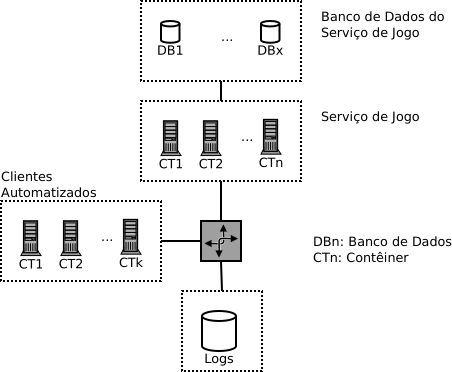
\includegraphics[height=6.5cm]{img/cap3/infraestrutura.png}
  \centering

  Fonte: O próprio autor.
\end{figure}



Como visível na Figura~\ref{Ambiente de testes}, o ambiente de testes planejado está organizado em cinco regiões.
%
Essas regiões foram segregadas com o objetivo de diminuir o impacto de desempenho e consumo de recursos por outras ferramentas durante a coleta de dados.
%
Por este motivo, as regiões da infraestrutura planejada são:



\begin{enumerate}
  \item \textbf{Serviço de Jogo}: A camada de serviço da infraestrutura dos testes concentrará a arquitetura dos microsserviços referente às arquiteturas de microsserviços analisadas.
  \item \textbf{Banco de dados do serviço de jogo}: A camada de banco de dados do serviço de jogo conterá os serviços de dados e web a fim de manter um padrão de banco de dados para ambos os serviços utilizados e auxiliar na inicialização dos testes.
  \item \textbf{Estresse}: A camada de estresse será responsável por realizar requisições ao serviço a fim de estressá-lo, simulando padrões de requisição de um padrão de um jogador.
  \item \textbf{Cliente}: A camada de cliente será composta pelos mesmos elementos da camada de estresse, porém em um ambiente controlado para que a suíte de estresse não interfira nas métricas obtidas no lado do cliente.
  \item \textbf{Dados}: A camada de dados será composta por um banco de dados de log a fim de armazenar os dados obtidos da camada Cliente e serviço, para utilizar na análise.
\end{enumerate}



Tais regiões da infraestrutura utilizada no ambiente de testes devem manter um padrão a fim que não exista interferência entre os testes, além do desempenho das arquiteturas do serviço.
%
Espera-se utilizar uma considerável parte do mesmo sistema de cliente para ambas as arquiteturas, excluindo-se os casos no quais a arquitetura necessite de alterações.
%
Nesse sentido, espera-se obter somente a interferência das arquiteturas expressa nos valores obtidos.



Para os casos de uso, serão utilizada as arquiteturas de microsserviços específicos a jogos \ac{mmorpg} obtidos da literatura.
%
São essas elas:



\begin{enumerate}
  \item \textbf{Arquitetura Rudy} (Subseção~\ref{rudy});
  \item \textbf{Arquitetura Salz} (Subseção~\ref{salz}); e
  \item \textbf{Arquitetura Willson} (Subseção~\ref{willson}).
\end{enumerate}



Tais arquiteturas vão impactar o serviço de jogo, banco de dados e as requisições a qual os clientes deverão realizar.
%
Espera-se obter os valores referente a diferença de consumo de recursos computacionais dentro de cenários controlados utilizando o ambiente de testes.



Com o objetivo de obter dados, se faz necessário estressar as arquiteturas em casos diferentes para garantir a confiabilidade dos dados obtidos.
%
Dessa forma, foi desenvolvido um cenário que comporte ambas as arquiteturas de microsserviços propostas a análise.
%
Este cenário possibilita a execução do experimento junto a simulação de clientes.



\subsection{Cenário}



O cenário reflete diretamente sobre o ambiente proposto para esta análise.
%
Ela será executada sobre 5 camadas, nas quais cada camada estará isolada em sub-redes em uma nuvem de computadores.

O cenário será composto por 5 sub-redes, na qual cada uma será responsável pela operação de uma região do ambiente planejado.
%
A visualização do cenário pode ser feita na Figura~\ref{fig:cenario}.

\begin{figure}[htb!]
  \caption{Cenário}
  \label{fig:cenario}
  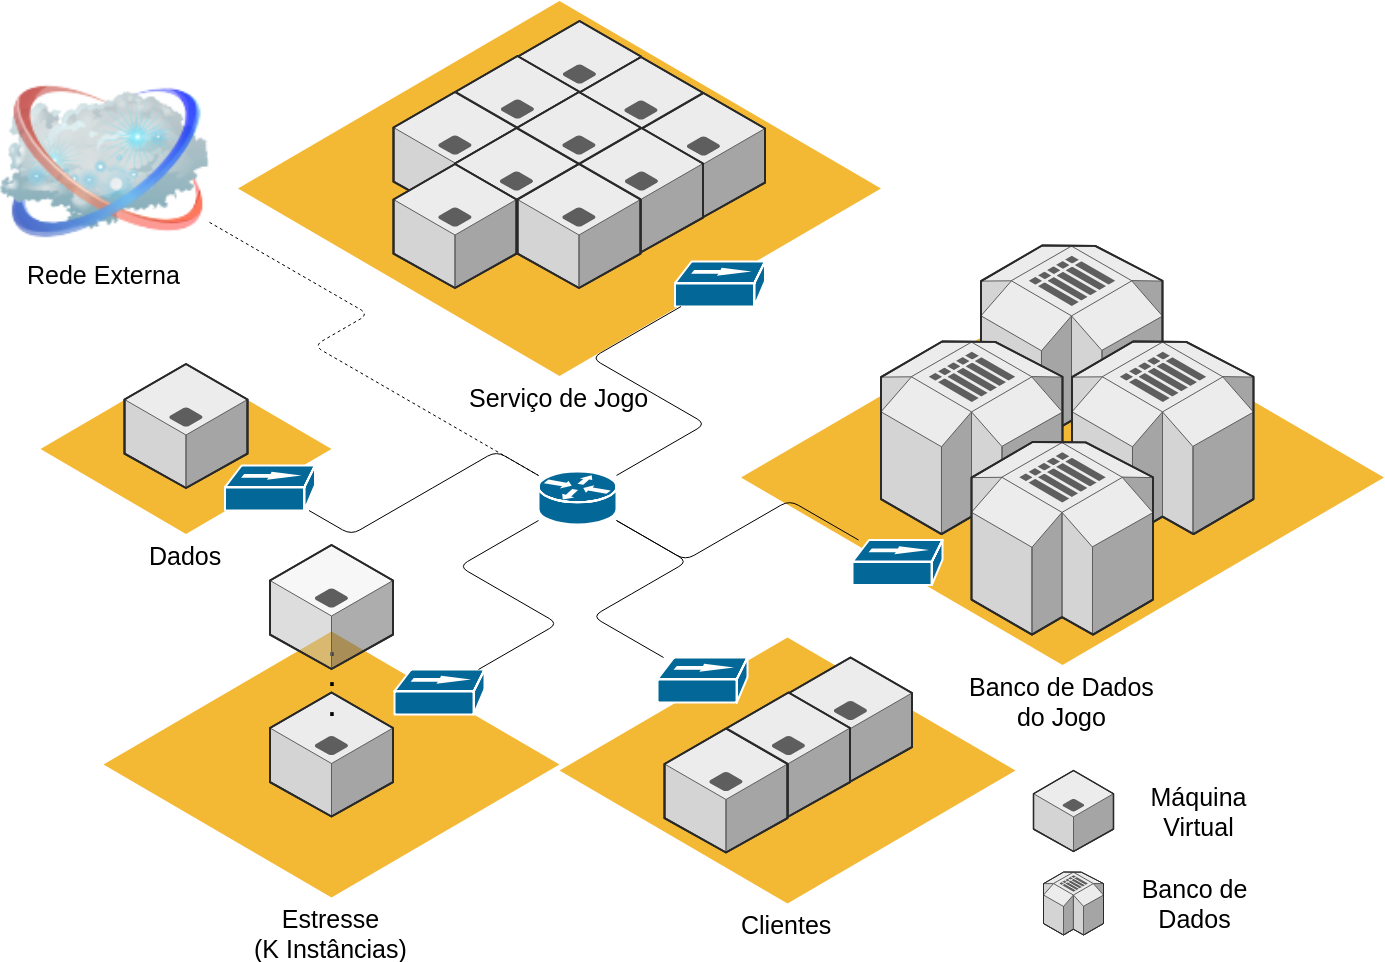
\includegraphics[height=8cm]{img/cap3/cenario.png}
  \centering

  Fonte: O próprio autor.
\end{figure}

O cenário, exibido na Figura~\ref{fig:cenario} descreve 5 sub-redes. Estas redes são descritas da seguinte forma:

\begin{enumerate}
  \item \textbf{Dados}: Armazena e processa os dados obtidos da arquitetura. É usado pelas redes \textit{Cliente} e \textit{Serviço de Jogo}.
  \item \textbf{Banco de dados do serviço de jogo}: Armazena dados do jogo. É usado pela rede \textit{Serviço de Jogo}.
  \item \textbf{Serviço de Jogo}: Executa sistemas \textit{web} e \ac{rpc} do serviço de jogo. Gera métricas para os serviços na rede \textit{Dados} e manipula os bancos de dados na rede \textit{Banco de dados do serviço de jogo}.
  \item \textbf{Estresse}: Executa múltiplos clientes, a fim de estressar o serviço de Jogo.
  \item \textbf{Clientes}: Executa um número controlado de clientes para obter métricas de tempo de resposta e latência entre as redes \textit{Cliente} e \textit{Serviço de Jogo}.
\end{enumerate}

Conforme a descrição de cada rede, existe uma interdependência dentre as redes.
%
Tal interdependência pode ser visualizada na Tabela~\ref{tab:interdependencia}.

\begin{table}[htb!]
\centering
\caption{Tabela de interdependência das sub-redes}
\label{tab:interdependencia}
\begin{tabular}{|l|l|l|l|l|l|}
\hline
\multicolumn{1}{|c|}{\rotatebox[origin=c]{-45}{Linha depende de Coluna}}  & \rotatebox[origin=c]{90}{Dados} & \rotatebox[origin=c]{90}{Banco de dados do serviço de jogo} & \rotatebox[origin=c]{90}{Serviço de Jogo} & \rotatebox[origin=c]{90}{Estresse} & \rotatebox[origin=c]{90}{Clientes} \\ \hline
Dados                             & --    & Não                               & Não             & Não      & Não      \\ \hline
Banco de dados do serviço de jogo & Não   & --                                & Não             & Não      & Não      \\ \hline
Serviço de Jogo                   & Sim   & Sim                               & --              & Não      & Não      \\ \hline
Estresse                          & Não   & Não                               & Sim             & --       & Não      \\ \hline
Clientes                          & Sim   & Não                               & Sim             & Não      & --       \\ \hline
\end{tabular}

Fonte: O próprio autor.
\end{table}

A Tabela~\ref{tab:interdependencia} refere-se a dependência das redes, conforme os serviços necessários para o seu funcionamento.
%
Dessa forma, espera-se bloquear o tráfego de pacotes entre redes que não são dependentes.

A implantação do serviço de jogo utilizará métodos de implantação de microsserviços, com ferramentas para gerenciamento de nós em uma rede de contêineres.
%
Por este motivo, todas as máquinas virtuais da rede \textit{Serviço de Jogo} terão os mesmos recursos, facilitando o comportamento do gerenciador ao escalar os serviços.

A implantação dos bancos de dados do serviço de jogo devem ser feitas diretas no sistema operacional da máquina virtual.
%
Dessa forma, segue-se uma boa prática de não armazenar dados dentro de contêineres.
%
Por sua vez, estas máquinas virtuais serão focadas em armazenamento.

A implantação dos clientes sobre a rede \textit{Clientes} executará um número limitado de contêineres fixo sobre as máquinas virtuais, para que não estresse as instâncias desta rede.
%
Nesse sentido, os recursos computacionais requiridos por estas instâncias são menores em relação aos demais.

A estrutura de implantação da rede \textit{Estresse} será dada por um gerenciador de nós em uma rede de contêineres.
%
Esta rede terá mais instâncias sob demanda conforme o caso de teste.

O limite de recursos do cenário é definido na Tabela~\ref{tab:limite_recursos}.
%
Nesta tabela também é definido a faixa de endereços de cada rede esperado.

\begin{table}[htb!]
\centering
\begin{adjustbox}{max width=\textwidth}
\caption{Limite de recursos por instância de cada rede}
\label{tab:limite_recursos}
\begin{tabular}{|l|l|l|l|l|l|}
\hline
Nome da Rede                      & Rede                     & Instâncias & Armazenamento / Ins. & N. Núcleos & Memória \\ \hline
\multicolumn{1}{|c|}{Dados}       & 10.0.*.* / 255.255.0.0   & 1          & 250GB                & 4          & 4GB     \\ \hline
Banco de dados do serviço de jogo & 10.51.*.* / 255.255.0.0  & 4          & 100GB                & 4          & 2GB     \\ \hline
Serviço de Jogo                   & 10.52.*.* / 255.255.0.0  & 10         & 25GB                 & 4          & 4GB     \\ \hline
Estresse                          & 10.100.*.* / 255.255.0.0 & N          & 25GB                 & 4          & 4GB     \\ \hline
Clientes                          & 10.101.*.* / 255.255.0.0 & 3          & 10GB                 & 2          & 1GB     \\ \hline
\end{tabular}
\end{adjustbox}

Fonte: O próprio autor.
\end{table}

A partir da Tabela~\ref{tab:limite_recursos}, espera-se definir um limite de recursos máximos utilizados pelo Serviço de Jogo.
%
A única rede que pode variar conforme o teste será a rede Estresse, visto que a demanda para estressar uma rede pode mudar conforme as características do teste.

Após ter definido as características básicas do cenário na qual será executado os experimentos, se faz necessário definir as características da simulação dos clientes para os experimentos.



\subsection{Simulação de Clientes}



Espera-se, utilizando a simulação de clientes, estressar as arquiteturas utilizando um ataque com \textit{bots}.
%
Neste cenário, para padronizar a coleta de dados, todos os \textit{bots} terão a mesma rotina evitando comportamento aleatório.



Porém, como requisito para se estipular as requisições, se faz obrigatório realizar um levantamento de requisitos na qual tanto o serviço quanto o cliente devem implementar.
%
Nesse sentido, a Tabela~\ref{tab:requisitos_funcionais} relaciona a funcionalidade com o impacto de implementação de tal funcionalidade.



\begin{table}[htb!]
\centering
\begin{adjustbox}{max width=\textwidth}
\caption{Requisitos funcionais e impacto de implementação}
\label{tab:requisitos_funcionais}
\begin{tabular}{|l|l|l|}
\hline
Requisito                                                       & Descrição                                                                                                                                                                                  & Implementação                                                                                                                                                                             \\ \hline
Identificação                                                   & \begin{tabular}[c]{@{}l@{}}Gera uma numeração única (token) com base\\ em uma tupla de dados.\end{tabular}                                                                                 & \begin{tabular}[c]{@{}l@{}}Será implementado utilizando algoritmo de hash (MD5),\\ de forma a garantir que este token seja único e diferente a\\ cada implementação.\end{tabular}         \\ \hline
Autenticação                                                    & \begin{tabular}[c]{@{}l@{}}Recebe o token e garante que não existe nenhuma\\ conexão utilizando o mesmo token.\end{tabular}                                                                & \begin{tabular}[c]{@{}l@{}}Será implementado usando um serviço de chave valor,\\ como o Redis.\end{tabular}                                                                               \\ \hline
\begin{tabular}[c]{@{}l@{}}Selecionar\\ Personagem\end{tabular} & \begin{tabular}[c]{@{}l@{}}Uma conexão deve requirir o controle de um\\ personagem.\end{tabular}                                                                                           & \begin{tabular}[c]{@{}l@{}}Será implementado utilizando uma árvore de cena interna\\ ao serviço, onde o tipo do nó será Personagem e o seu nome\\ será o nome do personagem.\end{tabular} \\ \hline
Chat                                                            & \begin{tabular}[c]{@{}l@{}}Será possível enviar mensagens e receber. Elas serão\\ baseadas na região. Será mantido uma distância fixa\\ para todos os casos de uso.\end{tabular}           & \begin{tabular}[c]{@{}l@{}}Deve existir uma estrutura de busca interna ao serviço para\\ consultar personagens de uma região em relação a um\\ usuário.\end{tabular}                      \\ \hline
Movimentar                                                      & \begin{tabular}[c]{@{}l@{}}Será possível movimentar o personagem para as\\ células adjacentes. Isso indica que o\\ posicionamento do personagem será baseado\\ em uma matriz.\end{tabular} & \begin{tabular}[c]{@{}l@{}}Esta ação deve comunicar a atualização para todos os demais\\ jogadores da região de interesse.\end{tabular}                                                   \\ \hline
Atacar                                                          & \begin{tabular}[c]{@{}l@{}}Ao atacar, o jogador causará um dano aleatório\\ baseado em seu nível em todos os inimigos das\\ células adjacentes.\end{tabular}                               & \begin{tabular}[c]{@{}l@{}}Esta ação irá manipular a árvore de objetos da cena do serviço\\ e deverá notificar todos os jogadores desta área de interesse.\end{tabular}                   \\ \hline
Consumir                                                        & \begin{tabular}[c]{@{}l@{}}Ao consumir um item, os atributos do personagem\\ serão alterados, influenciando na regra de negócio\\ utilizada nas arquiteturas de teste\end{tabular}         & \begin{tabular}[c]{@{}l@{}}Implicará na utilização de um banco de dados em memória\\ e manipulação de dados não visíveis pela\\ árvore de cena.\end{tabular}      \\ \hline
\end{tabular}
\end{adjustbox}

Fonte: O próprio autor.
\end{table}

A Tabela~\ref{tab:requisitos_funcionais} relata uma lista de funcionalidades mínimas que serão executadas na simulação.
%
A partir destas funcionalidades, pode-se definir quais requisições estarão disponíveis na \ac{api} para o cliente requisitar ao serviço.
%
A lista de comandos públicos é exibida na Tabela~\ref{tab:api_publica}.


\begin{table}[htb!]
\centering
\begin{adjustbox}{max width=\textwidth}
\caption{Requisitos mínimos para a implementação da simulação descrita}
\label{tab:api_publica}
\begin{tabular}{|l|l|l|l|l|}
\hline
Nome                  & Argumentos            & Retorno & Protocolo & Direção              \\ \hline
\textit{Auth}                  & \textit{Username, Password}    & \ac{json} & \textit{Web}       & Cliente para Serviço \\ \hline
\textit{CreateAccount}         & \textit{Username, Password}    & \ac{json} & \textit{Web}       & Cliente para Serviço \\ \hline
\textit{UpdateAccount}         & \textit{Username, Password}    & \ac{json} & \textit{Web}       & Cliente para Serviço \\ \hline
\textit{CreateCharacter}       & \textit{Token, Character Name} & \ac{json} & \textit{Web}       & Cliente para Serviço \\ \hline
\textit{DeleteCharacter}       & \textit{Token, Character ID}   & \ac{json} & \textit{Web}       & Cliente para Serviço \\ \hline
\textit{SelectCharacter}       & \textit{Token, Character ID}   & \ac{json} & \ac{rpc}           & Cliente para Serviço \\ \hline
\textit{WalkTo}                & \textit{Token, PosX, PosY}     &           & \ac{rpc}           & Cliente para Serviço \\ \hline
\textit{ConsumeItem}           & \textit{Token, Item}           &           & \ac{rpc}           & Cliente para Serviço \\ \hline
\textit{AtackHere}             & \textit{Token}                 &           & \ac{rpc}           & Cliente para Serviço \\ \hline
\textit{SendMessage}           & \textit{Token, Message}        &           & \ac{rpc}           & Cliente para Serviço \\ \hline
\textit{UpdateMapEstate}       & \textit{NPC, Action, MoreData} &           & \ac{rpc}           & Serviço para Cliente \\ \hline
\textit{UpdateCharacterEstate} & \textit{NPC, Action, MoreData} &           & \ac{rpc}           & Serviço para Cliente \\ \hline
\textit{ReceiveMessage}        & \textit{NPC, Message}          &           & \ac{rpc}           & Serviço para Cliente \\ \hline
\textit{ReBind}                & \textit{IP, Port}              &           & \ac{rpc}           & Serviço para Cliente \\ \hline
\end{tabular}
\end{adjustbox}
\end{table}

A Tabela~\ref{tab:api_publica} descreve todos os comando que estarão disponíveis na rede.
%
Além destes, serão implementados outros comandos para \ac{api} privada do serviço.
%
No entanto, os demais comandos da \ac{api} privada não serão utilizados pelo cliente, sendo necessariamente um requisito para o funcionamento do serviço com determinada arquitetura.


O ambiente da simulação será baseado em matrizes. Cada mapa pode ser visualizado como uma matriz de 100x100 unidades.
%
Os personagens podem locomover-se para as células adjacentes a sua localização.
%
O raio de interesse é de 4 células.
%
Um exemplo de estado do ambiente do jogo pode ser visualizado na Figura~\ref{fig:roi}.

\begin{figure}[htb!]
  \caption{Área de interesse da simulação com raio de 4 células}
  \label{fig:roi}
  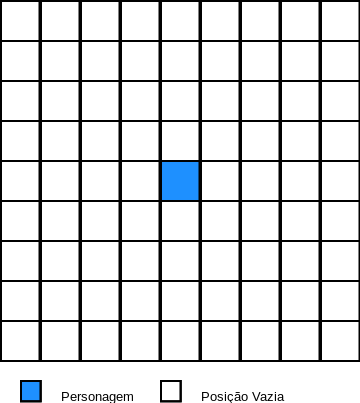
\includegraphics[height=5.0cm]{img/cap3/roi.png}
  \centering

  Fonte: O próprio autor.
\end{figure}

A partir da área de interesse do jogo, como o da Figura~\ref{fig:roi}, o \textit{bot} poderá decidir suas ações baseado em um automato.
%
Caso ele alcance os extremos do mapa, ele será movimentado para outro mapa.
%
Nos casos de arquiteturas com múltiplos gerenciadores de mundo, será utilizado o comando \textit{ReBind} para realizar a conexão com o microsserviço correto após o translado do personagem.



Todas as ações do \textit{bot} no mapa são baseado em um automato.
%
Nesse sentido, espera-se obter um padrão de movimentação a fim de evitar ciclos a qual um jogador comum dificilmente realizará (\textit{e.g.,} Andar para frente e para trás, ficar equipando itens em ciclo, ficar consumindo itens até acabar, \textit{etc.}).
%
A movimentação do personagem seguirá o automato descrito na Figura~\ref{fig:movimentacao}.


\begin{figure}[htb!]
  \caption{Automato de movimentação dos personagens simulados}
  \label{fig:movimentacao}
  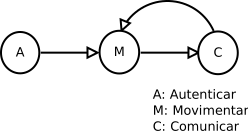
\includegraphics[height=3.5cm]{img/cap3/movimentacao.png}
  \centering

  Fonte: O próprio autor.
\end{figure}

A Figura~\ref{fig:movimentacao} descreve o comportamento de um \textit{bot} no ambiente do jogo simulado.
%
Ele seguirá um padrão de procurar batalhas, batalhar, gerenciar itens do personagem e buscar novas batalhas.
%
Este conjunto de ações simula o comportamento de busca de itens dentro de um jogo \ac{mmorpg}.
%
As características específicas de cada estado é definido da seguinte forma:

\begin{itemize}
  \item Autenticar: Realizará autenticação com o serviço \textit{web} ou \textit{rpc} apropriado a arquitetura. Neste passo o \textit{bot} receberá as informações do seu personagem.
  \item Buscar Inimigo: Caminhará de forma aleatória a fim de buscar um inimigo, caso não exista em sua área de interesse. Caso encontre em sua área de interesse, irá aproximar deste inimigo.
  \item Batalhar: Irá atacar um inimigo, aplicando dano a este \ac{npc}. O personagem poderá receber dano. Estes valores serão fixos baseados em seu equipamento. O personagem pode perder todos os seus pontos de vida, sendo desconectado do serviço.
  \item Gerenciar Itens: O \textit{bot} irá consumir itens para recuperar pontos de vida e usar equipamentos melhores aos já utilizados.
  \item Caminhar Aleatoriamente: O personagem caminhará aleatoriamente por um número de passos máximo. Após isso, voltará a buscar uma batalha.
\end{itemize}

Espera-se com esta sequência de ações, forçar aos \textit{bots} a explorar o cenário.
%
A cada mudança de estado, o jogador irá anunciar no chat a sua troca de ação.
%
Isso contribuirá com o monitoramento do comportamento dos personagens tanto quanto usará a funcionalidade de chat.
%
Para simular a ação de resposta de mensagens de um jogador, cada \textit{bot} que receber uma mensagem terá uma porcentagem fixa de $25\%$ responder a sua ação no atual momento.
%
Um \textit{bot} não poderá responder a uma mensagem na qual ele mesmo emitiu na região.


Ao realizar um \textit{ReBind} ou transitar de um mapa para o outro, o estado atual do automato volta para o estado \textbf{Autenticar}.
%
Caso já esteja autenticado, continuará a sua busca por inimigos na nova região.

O ambiente final da simulação tem 3 mapas no eixo horizontal e no eixo vertical, visto que esta é a combinação mínima para que o serviço tenha um mapa central com bordas para efetuar transições de novos personagens.

Após definido as características dos clientes simulados, pode-se definir os testes que serão executados sobre as arquiteturas de microsserviços específicos para jogos \ac{mmorpg}.

\subsection{Testes}

Os testes que serão executados no atual trabalho esperam analisar a quantia de recursos mínimos para executar os microsserviços e o crescimento de consumo de recursos conforme o crescimento de clientes simultâneos.
%
Nesse sentido, pode-se definir os seguintes testes:

\begin{enumerate}
  \item Executar a arquitetura Rudy com zero jogadores simultâneos, por 5 minutos;
  \item Executar a arquitetura Rudy com zero jogadores simultâneos, aumentando a cada minuto 10 jogadores ao serviço, até o serviço obter algum microsserviço terminar a sua execução por erro interno;
  \item Executar a arquitetura Salz com zero jogadores simultâneos, por 5 minutos;
  \item Executar a arquitetura Salz com zero jogadores simultâneos, aumentando a cada minuto 10 jogadores ao serviço, até o serviço obter algum microsserviço terminar a sua execução por erro interno;
  \item Executar a arquitetura Willson com zero jogadores simultâneos, por 5 minutos;
  \item Executar a arquitetura Willson com zero jogadores simultâneos, aumentando a cada minuto 10 jogadores ao serviço, até o serviço obter algum microsserviço terminar a sua execução por erro interno.
\end{enumerate}

A partir desta sequência de testes, espera-se obter valores suficientes para a análise das arquiteturas de microsserviços específico a jogos \ac{mmorpg}.

%ccm Genérico/abstratpo
% Quais experimentos serão realizados, se não necessário explicitar os caso de uso e o quê espera-se de resultado.
%
% Descrever como cenários, critérios e objetivos de testes.
